\documentclass[journal,10pt]{IEEEtran}

\usepackage{graphicx}
\usepackage{amsmath,amssymb,amsfonts}
\usepackage{booktabs}
\usepackage{url}
\usepackage[hidelinks]{hyperref}
\usepackage{textcomp}
\usepackage{bm}

\graphicspath{{figures/}}

\begin{document}

\title{Diabetic Foot Ulcers Severity Grading from Colour Wound
Images Using Deep Learning and Tissue Mapped Explainable AI}

\author{Mustapha~Nasser%
\thanks{M. Nasser is with the Faculty of Science and Technology,
American International University-Bangladesh, Dhaka, Bangladesh
(student ID 211002042).}}

\maketitle

\begin{abstract}
No public diabetic foot ulcer dataset carries severity annotation, so
recent work derives severity labels from image content. This paper
implements one such derivation, clustering wound pixels by colour and
thresholding the necrotic fraction, and then subjects the resulting
labels to four independent validation checks rather than assuming they
are correct. All four fail. Agreement with two clinicians is
indistinguishable from chance ($\kappa \approx 0$), against an
inter-rater agreement of $\kappa = 0.25$ that bounds what any automated
method could achieve. A negative control returns a severe grade for
60.2\% of lesion-free skin images. We identify the mechanism: $k$-means
with $k=3$ cannot express the absence of a tissue type, so the darkest
region of any image is labelled necrotic by construction, including
shadow, wound depth and darker skin. To separate label quality from
pipeline quality, the identical architecture and protocol are applied to
an expert-annotated infection task, used strictly as a control and not as
a substitute for severity, where the same code reaches AUROC 0.81.
Severity grading from colour wound images is therefore limited by the
absence of clinical annotation rather than by model capacity, and we
release the validation protocol that establishes this.
\end{abstract}

\begin{IEEEkeywords}
Diabetic foot ulcer, label validation, data leakage, negative control,
wound image analysis, ordinal regression, explainable AI.
\end{IEEEkeywords}

\section{Introduction}

\IEEEPARstart{D}{iabetes} mellitus affects a large and growing share of the
world population, and the International Diabetes Federation reported 537
million adults living with the disease in 2021, with projections reaching
783 million by 2045 \cite{idf2021}. Among its complications, diabetic foot
ulcers (DFU) carry the heaviest clinical and economic burden. Between 25\%
and 34\% of diabetic patients develop an ulcer during their lifetime
\cite{armstrong2017}, and more than 85\% of diabetes-related lower-limb
amputations are preceded by a foot ulcer \cite{pecoraro1990}. In
lower-middle-income countries the cost of treatment can reach several times
a patient's annual income \cite{cavanagh2012}.

Clinicians grade DFU severity using systems such as the Wagner scale
\cite{wagner1981} or the University of Texas classification
\cite{armstrong1998}, both of which map the wound to an ordinal category
that determines the treatment pathway. Assessment is performed by visual
inspection supported by physical probing, which introduces inter-clinician
variability and is unavailable in settings without wound care specialists
\cite{vannetten2020}. Automating this assessment from a photograph would
extend triage capacity to primary care and remote settings.

Deep learning has been applied to DFU image analysis since 2018
\cite{goyal2018}, and progress accelerated after the Diabetic Foot Ulcer
Challenge series introduced standardised benchmarks \cite{cassidy2021}. A
2025 systematic review screening 4{,}653 articles found that machine
learning models achieve accuracies between 0.88 and 0.97 on binary
detection and on infection or ischaemia classification \cite{gomes2025}.
Severity grading, however, remains unsolved on public data. Studies that
attempt Wagner grading rely on private hospital datasets that cannot be
reproduced \cite{zhou2025,abebe2025}, or collapse adjacent grades because
labelled data is insufficient \cite{zhou2025}.

The obstacle is not model capacity but annotation. No publicly downloadable
DFU dataset carries severity labels. A natural response, and the one this
work initially pursued, is to derive severity from image content: segment
the wound into tissue types by colour, compute the proportion of each, and
apply threshold rules anchored to published grading criteria. The approach
is attractive because it requires no clinician time and scales to any
unlabelled corpus.

This paper reports what happens when that derivation is validated rather
than assumed correct. It does not recover severity, and we document both
the evidence and the mechanism. To establish that the failure lies in the
labels and not in the surrounding pipeline, the same architectures and
evaluation protocol are applied to a wound classification task that does
carry expert annotation, where they perform as expected. The conclusion is
therefore specific: severity grading from colour wound images is not
blocked by model capacity or image resolution, but by the absence of
clinically annotated ground truth.

A second finding emerged from the same experiments. During the study we
designed TGO-Net, a tissue-guided architecture that injects the derived
tissue proportions into a frozen convolutional representation through a
learned multiplicative gate whose scalar is initialised at zero, so the
network reports for itself how much of that signal it uses. On the derived
labels the gated model appears to perform extremely well, but we show this
is circular: the tissue proportions are the label-generating variable. On
expert labels, where no such circularity exists, the gate never stabilises
and the gated model performs slightly worse than a plain CNN. The
architecture is retained in this paper as a diagnostic instrument rather
than a performance contribution, because the behaviour of its gate is
itself evidence about the labels.

The contributions of this work are:

\begin{itemize}
\item A \textbf{colour-based tissue proportion labelling method} that
derives mild, moderate and severe labels from wound images without
ground-truth annotations, specified in full so that it can be reproduced
and independently assessed.

\item A \textbf{four-part validation protocol} for derived image labels,
combining expert agreement, a negative control on lesion-free images, a
stability test across augmented copies of the same source photograph, and a
corpus plausibility check. Each check fails independently, and each is
inexpensive relative to the cost of training on invalid labels.

\item \textbf{Identification of the mechanism} behind the failure:
$k$-means with $k=3$ partitions every image into three non-empty clusters
and therefore cannot express the absence of necrosis; the assumed luminance
ordering of tissue types is inverted; and all dark image regions, including
darker skin, are absorbed into the cluster labelled necrotic.

\item A \textbf{leakage-free evaluation protocol} for pre-augmented corpora,
using dihedral-invariant content hashing, photograph-level identity
recovery from the union of filename and pixel evidence, and patient-grouped
folds verified on the image table across five independent keys.

\item \textbf{TGO-Net}, comprising a Tissue Proportion Encoder, a
Cross-Modal Gate with a zero-initialised scalar, and a rank-consistent
CORAL head, presented with its parameter budget and with the gate scalar
used as an interpretable measure of modality reliance.

\item A \textbf{control experiment} applying the identical architectures,
preprocessing and evaluation protocol to an expert-annotated infection
task, isolating label provenance as the cause of failure rather than model
capacity, input resolution or training configuration.
\end{itemize}

The remainder of this paper is organised as follows. Section II reviews
related work. Section III states the critical gaps in prior methods.
Section IV lists the core contributions. Section V describes the
methodology. Section VI details the datasets and experimental setup.
Section VII reports results. Section VIII discusses them. Sections IX
through XI state limitations, future work and conclusions.

\section{Related Work}

\subsection{Severity Grading from Wound Images}

The most direct prior work on Wagner grading from images is Zhou et al.
\cite{zhou2025}, who applied Mask2Former to segment seven tissue types and
assign grades on 671 annotated images from a Chinese hospital, reaching AUC
0.94 on tissue segmentation. Grades 1 and 2 were collapsed and grades 0 and
5 excluded because of insufficient samples, and the dataset is not public.
Abebe et al. \cite{abebe2025} applied MobileNetV2 to full six-class Wagner
grading on 3{,}700 images from three Ethiopian hospitals, reporting 82\%
validation accuracy, again on private data and without cross-dataset
validation. Anilkumar et al. \cite{anilkumar2026} compared six
architectures on a 407-image South Indian clinical dataset labelled by
IWGDF criteria, with MobileNetV2 reaching 82\% accuracy and adjacent-grade
confusion identified as the dominant failure mode. Wang et al.
\cite{wang2024score} proposed ScoreDFUNet, classifying images into ulcer,
infection, normal and gangrene zones on 1{,}426 images with 95.34\%
accuracy, without addressing the full severity scale.

The pattern across these studies is consistent: severity grading works when
clinicians have graded the images, and every such dataset is private. None
reports a protocol for deriving severity labels from public unlabelled
data, and none validates such labels.

\subsection{Architectures for DFU Classification}

The standard architecture shifted from custom convolutional networks to
pretrained backbones after the challenge series demonstrated that
fine-tuned EfficientNet models outperform task-specific designs on
infection and ischaemia classification \cite{liu2022}. Subsequent work has largely
pursued attention mechanisms and feature fusion on the same benchmarks:
transformer-attention hybrids \cite{karthik2025}, attention-driven dense networks
, reconstruction residual networks with spatial-channel attention
\cite{wang2024farr}, handcrafted texture descriptors combined with learned embeddings
\cite{algaraawi2022}, and patch-based networks with context-preserving attention \cite{liu2021}.
Reported macro F1 on the DFUC-2021 infection and ischaemia task
clusters around 80\%.

These studies share a limitation relevant here: all evaluate on labels
supplied with the dataset, and none reports whether augmented copies of the
same photograph, or multiple wound sites from the same patient, were
separated across training and test splits.

\subsection{Explainability in DFU Models}

Explainability work in this domain applies SHAP, LIME and Grad-CAM to
binary detection, reporting high accuracies and heatmaps that localise
the ulcer region \cite{rathore2025,mahmud2025}. A recent
review found that only 23\% of DFU studies incorporate explainability
methods at all, and that none maps activation outputs to clinical wound
tissue features \cite{liu2025review}.

Across this literature, explainability outputs are generated at the
detection level and are not linked to validated tissue references. Our
analysis in Section VII-E addresses why doing so is harder than it appears
when the tissue reference is itself derived by clustering.

\subsection{Label Quality and Data Leakage in Medical Imaging}

Concern about label quality and evaluation integrity is not specific to
DFU. Reviews of machine learning in medical imaging repeatedly identify
optimistic evaluation arising from improper data partitioning, in
particular when multiple images originate from the same patient or the same
acquisition \cite{yap2021,silva2025}. Gomes et al. \cite{gomes2025} note
that only 67.3\% of DFU classification datasets are publicly accessible,
which limits independent verification of both labels and splits. Dhar et
al. \cite{dhar2024} report a pilot study on wound tissue segmentation and
observe that inter-annotator variation is substantial even among trained
annotators, which is consistent with the inter-rater agreement we measure
in Section VII-A.

To our knowledge no prior DFU study reports a negative control on
lesion-free images, or a stability analysis across augmented copies of the
same photograph, as a precondition for trusting derived labels.

\section{Critical Gaps and Limitations of Prior Methods}

Four gaps follow from the literature above, and the contributions in
Section IV map onto them one to one.

\textbf{Gap 1: derived labels are used without validation.} Where public
data lacks severity annotation, labels are derived from image content and
then used directly for training. No prior study reports whether the derived
labels agree with clinicians, whether they behave correctly on images
containing no lesion, or whether they are stable under transformations that
do not change the clinical picture. Contribution 2 supplies a validation
protocol; contribution 3 reports the mechanism when it fails.

\textbf{Gap 2: evaluation integrity on pre-augmented corpora is not
reported.} Public wound corpora are frequently distributed after
augmentation, so a split over image files does not separate photographs.
None of the reviewed studies states how augmented copies or per-patient
multiplicity were handled. Contribution 4 supplies a protocol that
addresses this and verifies it on the image table rather than on an
aggregated table.

\textbf{Gap 3: architectural additions are not tested against a
label-quality confound.} Where auxiliary features derived from the same
images are added to a network, an improvement may reflect the auxiliary
feature carrying label information rather than clinical signal.
Contribution 5 introduces an architecture whose gate scalar makes modality
reliance directly readable, and contribution 6 supplies the control
condition needed to interpret it.

\textbf{Gap 4: no control separates label quality from pipeline quality.}
When a method underperforms, the literature does not distinguish between
inadequate labels and an inadequate model. Contribution 6 applies the
identical pipeline to an expert-annotated task on comparable images,
isolating the variable.

\section{Core Contributions}

The contributions listed in Section~I are developed as follows: the
labelling method in Section~V-B, the validation protocol in Section~V-C
with results in Section~VII-A, the mechanism in Section~VII-B, the
evaluation protocol in Section~V-D, TGO-Net in Sections~V-E and~V-F, and
the control experiment in Section~VII-C.

% ---------------------------------------------------------------------
% FIGURE 1 — pipeline overview (full width, top of page)
% ---------------------------------------------------------------------
\begin{figure*}[!t]
\centering
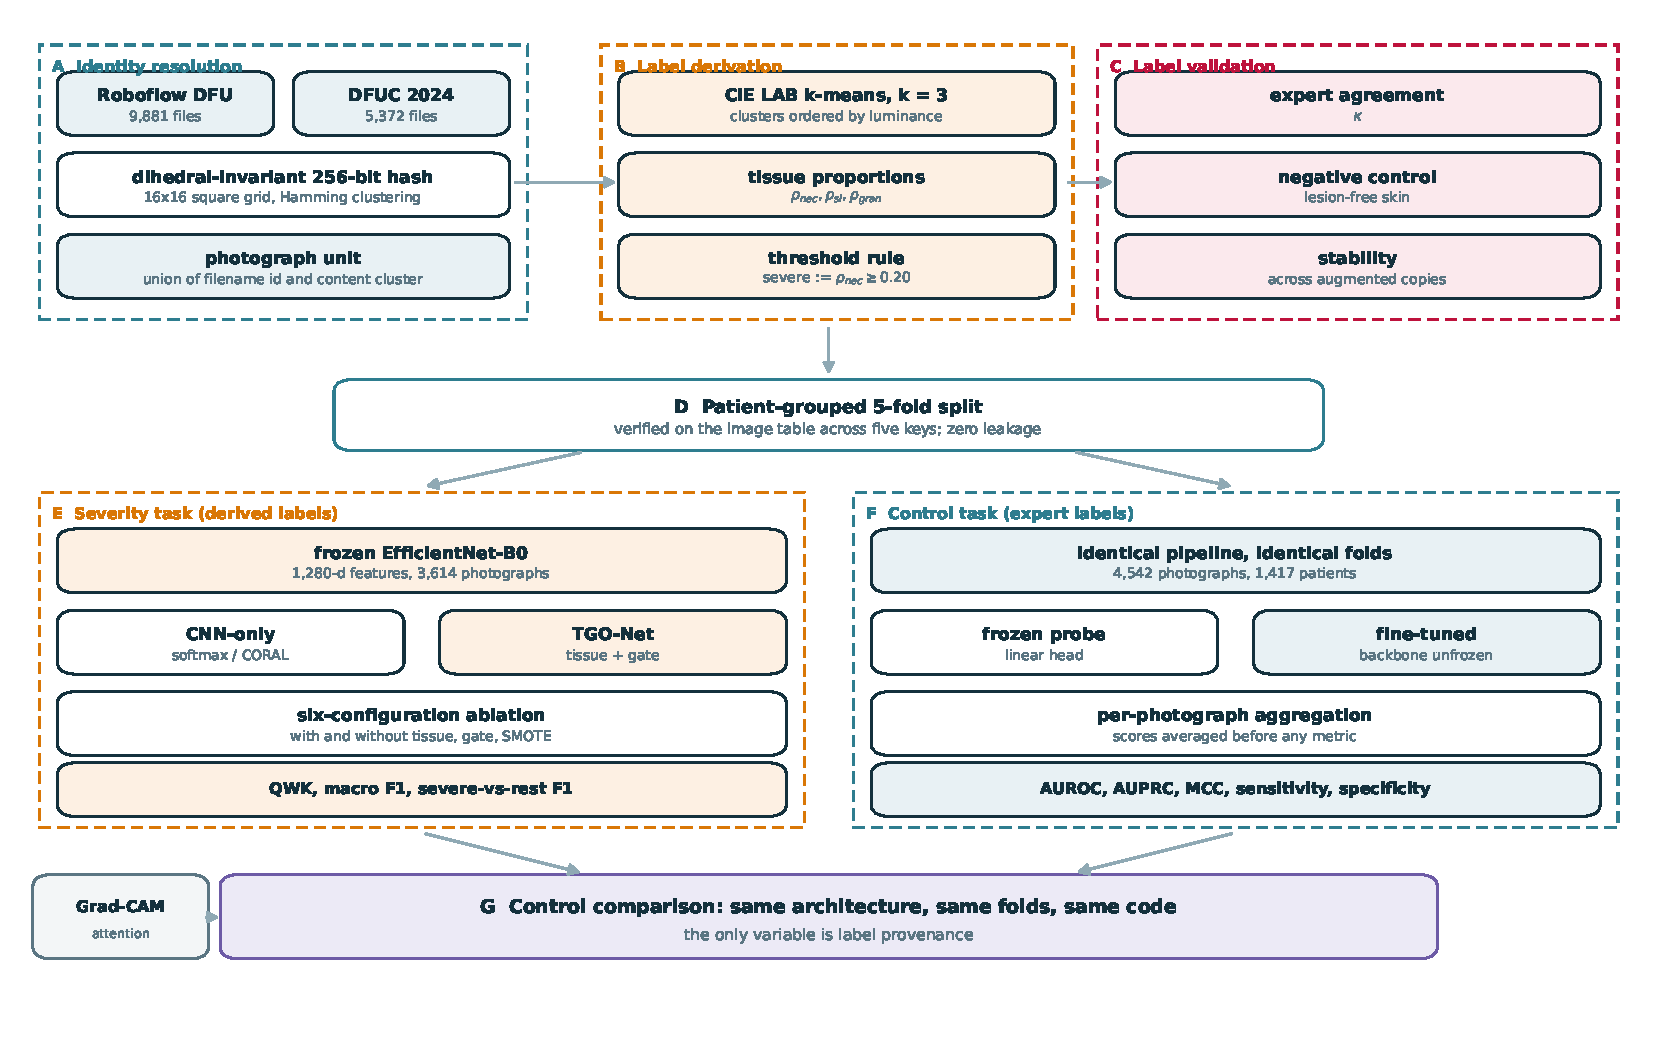
\includegraphics[width=\textwidth]{fig_pipeline.pdf}
\caption{End-to-end pipeline. Stage A resolves photograph and patient
identity from the union of filename and pixel evidence. Stage B derives
severity labels by colour clustering. Stage C validates those labels
against four independent checks and consolidates them to one label per
photograph. Stage D builds patient-grouped folds and verifies zero leakage
on the image table. Stages E and F train identical architectures on derived
and expert labels respectively, using the same folds and the same code.
Stage G compares them, isolating label provenance as the only variable.}
\label{fig:pipeline}
\end{figure*}

\section{Proposed Methodology}

The pipeline comprises seven stages: identity resolution, label derivation,
label validation, split construction, feature extraction, model training
with ablation, and statistical analysis. Each stage writes an artefact
consumed by the next, and each asserts its preconditions before running, so
that a stage cannot silently operate on incomplete input.

\subsection{Pipeline Overview}

Fig.~\ref{fig:pipeline} shows the end-to-end dataflow. Two corpora enter
stage A, where every image receives a photograph identifier and a patient
identifier. Stage B derives severity labels on the first corpus. Stage C
validates those labels and consolidates them to one label per photograph.
Stage D constructs patient-grouped folds and verifies that no identity key
spans a fold boundary. Stages E and F train models on the derived labels
and on expert labels respectively, using the same folds and the same code.
Stage G compares the two.

For an image $I$, the forward pass through the model is

\begin{equation}
\begin{aligned}
z    &= \phi_{\text{B0}}(I), \quad z \in \mathbb{R}^{1280}, \\
p    &= \big(\rho_{\text{nec}}, \rho_{\text{sl}}, \rho_{\text{gran}}\big)
        \in \Delta^{2}, \\
e    &= \psi(p), \quad e \in \mathbb{R}^{64}, \\
\tilde{z} &= z \odot \big(1 + \gamma \tanh(W_g e + b_g)\big), \\
\eta &= \mathcal{H}(\tilde{z}),
\end{aligned}
\label{eq:forward}
\end{equation}

where $\phi_{\text{B0}}$ is a frozen EfficientNet-B0 backbone \cite{tan2019} with its
classification head removed, $\psi$ is the Tissue Proportion Encoder,
$\Delta^{2}$ is the two-dimensional probability simplex, $\odot$ denotes
elementwise multiplication, $\gamma \in \mathbb{R}$ is a single learned
scalar, and $\mathcal{H}$ is a task-specific head. Section V-E describes
each component and Section V-F formalises them.

\subsection{Severity Label Derivation}

Because no public DFU corpus carries severity annotation, labels are
derived from tissue composition. Each image is resized to $128 \times 128$
and converted from RGB to CIE LAB, which separates luminance from
chrominance and reduces the effect of illumination differences between
sources. The wound pixel set is partitioned by $k$-means with $k = 3$,
using four initialisations. Clusters are ordered by the $L^{*}$ coordinate
of their centroids so that a given proportion index refers to the same
quantity in every image, and are assigned to necrotic, slough and
granulation tissue in ascending order of luminance, following the
convention that necrotic tissue is darkest and granulation lightest.

The tissue proportion for type $t$ is

\begin{equation}
\rho_t = \frac{|C_t|}{\sum_{j=1}^{3} |C_j|},
\qquad \sum_t \rho_t = 1,
\label{eq:props}
\end{equation}

where $C_t$ is the set of pixels assigned to cluster $t$. Severity is then
assigned by threshold rules anchored to published grading descriptions:

\begin{equation}
s =
\begin{cases}
\text{severe}   & \text{if } \rho_{\text{nec}} \geq 0.20, \\[2pt]
\text{mild}     & \text{if } \rho_{\text{gran}} \geq 0.67
                   \ \wedge\ \rho_{\text{sl}} \leq 0.27, \\[2pt]
\text{moderate} & \text{otherwise.}
\end{cases}
\label{eq:rule}
\end{equation}

Two implementation details are load-bearing. Reducing the number of
$k$-means initialisations to one shifts individual proportions by up to
0.166 relative to a ten-initialisation reference, which is the same order
as the effect being measured, so four initialisations are retained.
Ordering clusters by luminance is required because $k$-means returns
clusters in arbitrary order; without it the proportion vector is
meaningless across images.

\subsection{Label Validation Protocol}

A derived label is only useful if it recovers the quantity it claims to.
Four checks are applied, each capable of failing independently.

\emph{Expert agreement} compares derived grades against clinician review on
a stratified sample, reporting Cohen's $\kappa$ against each reviewer and
between reviewers. The inter-rater value is essential context: it bounds
what agreement any automated method could plausibly achieve.

\emph{Negative control} applies the identical derivation to images
containing no ulcer. The correct necrotic fraction for intact skin is zero,
so any severe grade is a false positive that the method cannot detect on
wound images, where no reference value exists.

\emph{Stability} groups images by source photograph and asks whether a
photograph's own augmented copies receive the same grade. Augmentation does
not change the clinical picture, so disagreement indicates that the label
is determined by something other than wound appearance.

\emph{Plausibility} compares the resulting class distribution against the
composition of clinical cohorts.

\subsection{Leakage-Free Evaluation Protocol}

Public wound corpora are frequently distributed after augmentation, so a
split over image files does not separate photographs. The protocol treats
evaluation identity and split grouping as separate problems.

Photograph identity is the union of two signals. Filenames encode the
source photograph through export and augmentation suffixes, and pixel
content is summarised by a perceptual hash made invariant to rotation and
mirroring, then compared by Hamming distance rather than equality so that
re-encoding does not split a photograph from its own copies. Neither
signal alone suffices: hashing over-splits copies whose appearance
diverges, and filenames are renumbered between exports. Two images
therefore belong to the same photograph unit if they share either
signal, computed as connected components over the union of both
relations. Implementation details are given in the released notebooks.

The split group is deliberately more conservative than the evaluation unit:
patients joined by any shared content cluster are placed in the same group,
including false-positive links, because an unnecessary merge costs less
than a leak. Folds are stratified over these groups.

Verification runs on the full image table rather than an aggregated table,
across five keys: patient, photograph, unit, group and content cluster. An
aggregated table hides patients dropped by first-match merges, and an
earlier version of this check reported success while two patients genuinely
spanned folds.

Finally, predictions are made per image and averaged to one score per
photograph before any metric is computed. Without this step a photograph
with eight augmented copies contributes eight times and one with a single
copy contributes once, which weights the test set toward heavily augmented
cases.

\subsection{TGO-Net Architecture}

Fig.~\ref{fig:arch} shows the architecture. The tissue proportions computed
during labelling are unused by a standard convolutional network, which sees
only pixels. TGO-Net supplies them as a second input stream while keeping
the backbone frozen, which keeps training feasible without sustained
accelerator access and makes every reported figure a linear probe on fixed
features rather than a tuned ceiling.

\textbf{Tissue Proportion Encoder.} The three-dimensional proportion vector
is lifted to a 64-dimensional embedding by a two-layer perceptron with GELU
activation \cite{hendrycks2016} and layer normalisation \cite{ba2016}.
Layer normalisation is used rather than batch normalisation because batch
statistics over a three-dimensional input are unstable at small batch
sizes. This component holds 2{,}432 parameters.

\textbf{Cross-Modal Gate.} The embedding is converted into a per-channel
multiplier on the frozen feature. The scalar $\gamma$ is initialised at
zero, so at initialisation $\tilde{z} = z$ and the model is exactly the
frozen-CNN baseline; the tissue pathway must earn any influence through
training. This makes $\gamma$ a directly interpretable measure of how much
the network relies on tissue composition relative to appearance. The
hyperbolic tangent bounds each channel's scaling to
$(1 - |\gamma|,\ 1 + |\gamma|)$. Multiplicative fusion is used rather than
concatenation because a 64-dimensional signal concatenated to 1{,}280
dimensions can be ignored through near-zero weights; the concatenation
variant is retained as an ablation so that this choice is tested rather
than asserted. This component holds 83{,}201 parameters.

\textbf{Prediction heads.} For the three-class ordinal formulation the head
is CORAL \cite{cao2020}: a single shared weight vector with $K-1$
independent bias terms. Because the weight vector is shared and only the
biases differ, the logits differ by a constant for every input and cannot
cross, so the model is structurally incapable of asserting
$P(y > \text{moderate}) > P(y > \text{mild})$. Rank consistency is
guaranteed by the architecture rather than encouraged by the loss. For the
binary formulation the head is a single logit.

Total trainable parameters are 86{,}915 for the ordinal head and 86{,}914
for the binary head, against 5{,}288{,}548 parameters in the frozen
backbone, so 1.62\% of the model is trained.

\subsection{Mathematical Formulation}

The Tissue Proportion Encoder maps $p \in \Delta^{2}$ to $e$ by

\begin{equation}
e = \sigma_{\text{G}}\Big(
    \mathrm{LN}\big(W_2\,
    \sigma_{\text{G}}(\mathrm{LN}(W_1 p + b_1))
    + b_2\big)\Big),
\label{eq:encoder}
\end{equation}

where $W_1 \in \mathbb{R}^{32 \times 3}$,
$W_2 \in \mathbb{R}^{64 \times 32}$, $\mathrm{LN}$ denotes layer
normalisation and $\sigma_{\text{G}}$ the GELU nonlinearity.

The Cross-Modal Gate produces a bounded per-channel modulation

\begin{equation}
g = \tanh(W_g e + b_g), \qquad
\tilde{z} = z \odot (1 + \gamma g),
\label{eq:gate}
\end{equation}

with $W_g \in \mathbb{R}^{1280 \times 64}$ and $\gamma \in \mathbb{R}$
initialised at $0$. Because $g \in (-1, 1)^{1280}$, each channel of $z$ is
scaled within $(1 - |\gamma|,\ 1 + |\gamma|)$, so a large $\gamma$ is
required before the tissue stream can materially alter the representation.

The CORAL head produces $K-1$ ordered logits from a shared projection

\begin{equation}
\eta_k = w^{\top} \tilde{z} + b_k, \qquad k = 1, \dots, K-1,
\label{eq:coral}
\end{equation}

trained against binary targets $y_k = \mathbb{1}[y > k]$ with

\begin{equation}
\mathcal{L}_{\text{CORAL}} = -\sum_{k=1}^{K-1}
\Big[ y_k \log \varsigma(\eta_k)
    + (1 - y_k) \log\big(1 - \varsigma(\eta_k)\big) \Big],
\label{eq:coralloss}
\end{equation}

where $\varsigma$ is the logistic function. The predicted class is
$\hat{y} = \sum_{k} \mathbb{1}[\varsigma(\eta_k) > 0.5]$. For the binary
task the objective is weighted cross-entropy

\begin{equation}
\mathcal{L}_{\text{BCE}} = -\big[ w^{+} y \log \varsigma(\eta)
    + (1-y) \log(1 - \varsigma(\eta)) \big],
\label{eq:bce}
\end{equation}

with $w^{+} = n_{-} / n_{+}$ computed on the training split of each fold.

Where class imbalance is addressed by resampling, SMOTE \cite{chawla2002}
is applied to the concatenated vector $[\,z \mid p\,]$ of the training
split rather than to features alone. A convex combination of two points of
$\Delta^{2}$ remains in $\Delta^{2}$, so interpolated tissue vectors stay
valid proportions:

\begin{equation}
\tilde{p} = \lambda p_a + (1-\lambda) p_b \in \Delta^{2},
\qquad \lambda \sim U(0,1).
\label{eq:smote}
\end{equation}

\subsection{Explainability}

Grad-CAM \cite{selvaraju2020} is computed on the last convolutional block.
For class score $y^{c}$ and feature maps $A^{k}$,

\begin{equation}
\alpha^{c}_{k} = \frac{1}{Z}\sum_{i}\sum_{j}
\frac{\partial y^{c}}{\partial A^{k}_{ij}},
\qquad
L^{c} = \mathrm{ReLU}\Big(\sum_{k} \alpha^{c}_{k} A^{k}\Big).
\label{eq:gradcam}
\end{equation}

The fraction of activation falling inside a tissue cluster mask $M^{c}$ is

\begin{equation}
A^{c}_{\text{align}} =
\frac{\sum_{ij} L^{c}_{ij} M^{c}_{ij}}{\sum_{ij} L^{c}_{ij}}.
\label{eq:align}
\end{equation}

Because a cluster covering a larger share of the image absorbs more
activation by area alone, we report the area-normalised lift
$A^{c}_{\text{align}} / \bar{M}^{c}$, where $\bar{M}^{c}$ is the fraction
of pixels in the mask. A lift of $1.0$ indicates attention proportional to
cluster size and therefore no preferential targeting. Section VII-E states
what this quantity can and cannot support.


% ---------------------------------------------------------------------
% FIGURE 2 — TGO-Net architecture (full width)
% ---------------------------------------------------------------------
\begin{figure*}[!t]
\centering
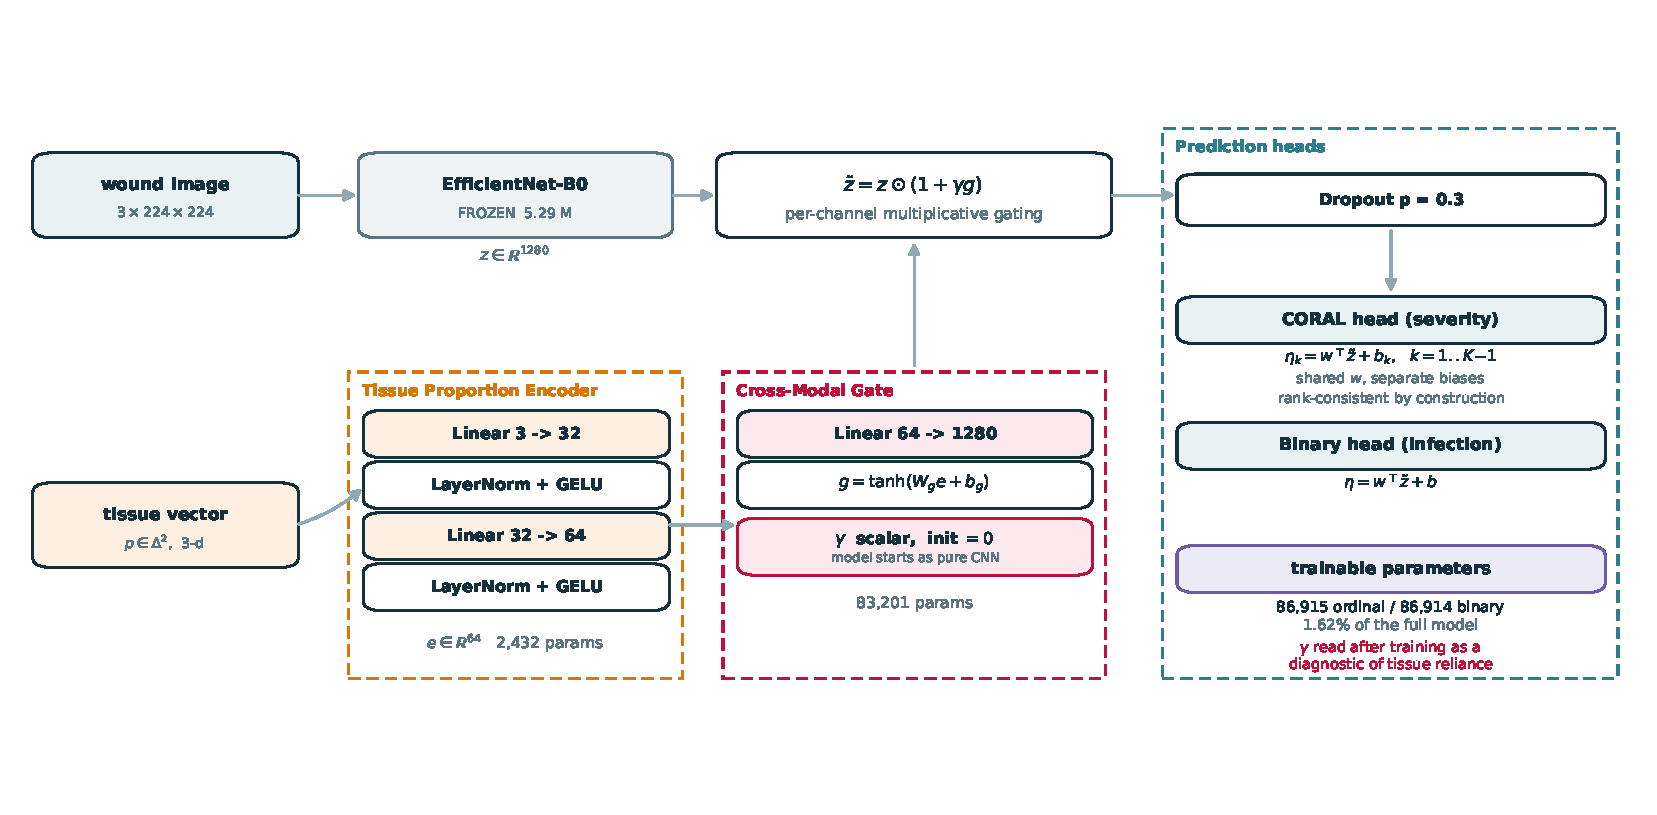
\includegraphics[width=\textwidth]{fig_architecture.pdf}
\caption{TGO-Net architecture. A frozen EfficientNet-B0 produces a
1{,}280-dimensional appearance feature. The Tissue Proportion Encoder lifts
the three-dimensional tissue vector to a 64-dimensional embedding using
layer normalisation, which is stable at small batch sizes where batch
statistics over three inputs are not. The Cross-Modal Gate converts that
embedding into a bounded per-channel multiplier scaled by a single learned
scalar $\gamma$ initialised at zero, so the model begins as the frozen-CNN
baseline and the tissue pathway must earn any influence. The CORAL head
shares one weight vector across $K-1$ ordered biases, making rank
consistency structural rather than loss-encouraged. Trainable parameters
total 86{,}915, or 1.62\% of the full model.}
\label{fig:arch}
\end{figure*}

\section{Experimental Setup}

\subsection{Datasets}

Three publicly accessible sources are used, summarised in
Table~\ref{tab:datasets}. All are downloadable without credentialing.

The \textbf{Roboflow DFU} corpus \cite{roboflow_dfu} supplies 9{,}881 labelled images and is
the subject of the derivation study. Content-based grouping reduces it to
3{,}614 source photographs, a property not visible from the file listing
and central to the leakage analysis. It is available at
\url{https://universe.roboflow.com/ssk-r6ppk/diabetic-ulcers}.

The \textbf{Kaggle DFU} dataset \cite{alzubaidi2020} contributes 543
lesion-free skin patches at $224 \times 224$ pixels, used exclusively as
the negative control. No image from this source enters training.

\textbf{DFUC 2024} \cite{dfuc2024} provides the expert-annotated infection task used for
the control experiment, accessed at
\url{https://universe.roboflow.com/wed-axnxx/dfuc-2024}. Its 5{,}372
infection-axis images resolve to 4{,}542 evaluation units from 1{,}417
patients after conflict removal, with 2{,}767 infected and 2{,}605 not
infected, a ratio of $1.06:1$.

Content comparison between the two wound corpora finds 14 shared
photographs, corresponding to 0.2\% of Roboflow and 0.3\% of DFUC, so the
control task is effectively independent of the derivation study.

\begin{table}[!t]
\caption{Dataset summary after content-based deduplication}
\label{tab:datasets}
\centering
\small
\begin{tabular}{@{}llrr@{}}
\toprule
Dataset & Role & Files & Photographs \\
\midrule
Kaggle DFU   & Negative control    & 543      & --      \\
Roboflow DFU & Severity derivation & 9{,}881  & 3{,}614 \\
DFUC 2024    & Control experiment  & 5{,}372  & 4{,}542 \\
\bottomrule
\end{tabular}
\end{table}

Consolidation to one label per photograph yields 30 mild, 1{,}235 moderate
and 2{,}349 severe cases (Fig.~\ref{fig:classes}). The mild class amounts
to approximately six
photographs per fold, which is discussed in Section IX.

\subsection{Implementation and Hardware}

Experiments ran on Google Colab with an NVIDIA Tesla T4 (16\,GB) and, for
non-accelerated stages, on an Apple Silicon workstation using the Metal
Performance Shaders backend. Software: Python 3.10, PyTorch 2.x
\cite{paszke2019}, torchvision, scikit-learn \cite{pedregosa2011},
scikit-image, imbalanced-learn. Hyperparameters are listed in
Table~\ref{tab:hyper}. Mixed precision is enabled on CUDA only.

\begin{table}[!t]
\caption{Training configuration}
\label{tab:hyper}
\centering
\small
\begin{tabular}{@{}ll@{}}
\toprule
Setting & Value \\
\midrule
Backbone            & EfficientNet-B0, ImageNet weights \\
Backbone state      & frozen (unfrozen in Section VII-D) \\
Input size          & $224 \times 224$ RGB \\
Optimiser           & Adam ($10^{-3}$), AdamW ($3\times10^{-5}$) \\
Weight decay        & $10^{-4}$ \\
Batch size          & 256 (probe), 32 (fine-tune) \\
Max epochs          & 60 (probe), 8 (fine-tune) \\
Early stopping      & patience 12 (probe), 3 (fine-tune) \\
Dropout             & 0.3 \\
Tissue encoder      & $3 \to 32 \to 64$, GELU, LayerNorm \\
Gate init $\gamma$  & 0.0 \\
Trainable params    & 86{,}915 ordinal / 86{,}914 binary \\
Cross-validation    & 5-fold, patient-grouped \\
Random seed         & 42 \\
$k$-means           & $k=3$, 4 initialisations, LAB \\
\bottomrule
\end{tabular}
\end{table}

\subsection{Evaluation Metrics}

For the ordinal severity task we report quadratic weighted kappa (QWK),
which penalises distant misgradings more than adjacent ones and is standard
for ordinal clinical scales; macro F1; mean absolute error in grade units;
and a collapsed severe-versus-rest F1, which is the only per-class quantity
the mild sample size supports.

For the binary infection task we report AUROC and AUPRC, which are
threshold-free; Matthews correlation coefficient, which uses all four
confusion-matrix cells and cannot be inflated by the majority class;
sensitivity and specificity separately, because missing an infection and
over-calling one carry different clinical costs; and balanced accuracy.
Every metric is computed on photograph-level scores.

Confidence intervals are percentile bootstrap over folds with 2{,}000
resamples. Paired comparisons across the shared folds use a paired
$t$-test, and the family of tissue-pathway tests is corrected by the
Holm-Bonferroni procedure \cite{holm1979}.

\subsection{Code Availability}

Source code is not publicly available at time of submission. The pipeline
is implemented as eleven sequential notebooks, each asserting its inputs
and writing artefacts consumed by the next, so that every reported value
traces to a specific executed cell.

\section{Results}

\subsection{Label Validation}

Table~\ref{tab:validation} reports the four checks and Fig.~\ref{fig:valid}
summarises three of them. All four fail.

\begin{table}[!t]
\caption{Label validation. Four independent checks, all failing.}
\label{tab:validation}
\centering
\small
\begin{tabular}{@{}llr@{}}
\toprule
Check & Measure & Result \\
\midrule
Expert agreement & derived vs.\ reviewer A & $-0.0254$ \\
Expert agreement & derived vs.\ reviewer B & $+0.0359$ \\
Expert agreement & reviewer A vs.\ B       & $+0.2537$ \\
\midrule
Negative control & lesion-free graded severe & 60.2\% \\
Negative control & max necrosis, intact skin & 0.570 \\
\midrule
Stability & photographs with $>1$ grade & 61.7\% \\
\midrule
Plausibility & mean necrotic fraction     & 0.231 \\
Plausibility & images above severe cut    & 63.1\% \\
\bottomrule
\end{tabular}
\end{table}

\emph{Expert agreement.} On 134 matched images, agreement between the
derived grade and reviewer A was $\kappa = -0.025$, and against reviewer B
$\kappa = +0.036$. Both are indistinguishable from chance. The two
reviewers agreed with each other at $\kappa = 0.254$, which is fair on the
Landis and Koch scale \cite{landis1977}. That value is the relevant
ceiling: severity grading from a photograph is a genuinely difficult task
on which trained clinicians agree only moderately, and the derived labels
do not approach even that level.

\emph{Negative control.} Applied to 543 lesion-free skin images, the
derivation returned a severe grade for 60.2\% of them, with a mean necrotic
fraction of 0.222 and a maximum of 0.570 on intact tissue. The correct
value in every case is zero. These images are out of domain by design; the
purpose of a negative control is not to measure performance but to observe
behaviour where ground truth is known. The same contamination is present in
wound images, where it cannot be detected because no reference exists.

\emph{Stability.} Of 2{,}818 photographs with more than one augmented copy,
1{,}739 (61.7\%) received more than one severity grade across copies of
themselves. Augmentation does not change the wound, so a label that changes
under augmentation is not measuring the wound.

\emph{Plausibility.} The corpus mean necrotic fraction is 0.231 and 63.1\%
of images exceed the severe threshold. No clinical DFU cohort is
approximately two-thirds severe.

\subsection{Mechanism}

Three mechanisms explain these results, each sufficient alone.

First, $k$-means with $k = 3$ partitions every image into three non-empty
clusters whose proportions sum to one. There is no output corresponding to
``no necrosis present''. The darkest third of the pixel distribution is
labelled necrotic by construction, whatever the image contains. This is why
lesion-free skin receives a severe grade.

Second, the assumed luminance ordering is inverted. Cross-referencing
against tissue references places granulation near $L^{*} = 118$ and
periwound callus near $L^{*} = 168$: granulation is darker than callus,
the opposite of the ordering the derivation assumes when it assigns the
highest-luminance cluster to granulation.

Third, all dark regions fall into the same cluster: shadow, wound depth,
hair, image background and darker skin. Fitzpatrick phototypes V and VI
\cite{fitzpatrick1988} overlap the necrosis reference range in LAB space,
so the method over-grades darker skin systematically. This is a fairness
concern as well as a validity one, and it would not be visible in aggregate
accuracy on a predominantly light-skinned cohort.

\subsection{Control Experiment}

The results above show that the derived labels do not recover severity.
They do not by themselves show that the labels are the only problem. To
separate label quality from pipeline quality, the identical architecture,
preprocessing and evaluation protocol were applied to the DFUC 2024
infection task, which carries clinician annotation.

Infection and severity are different constructs and this paper does not
treat them as interchangeable. Infection is one of several criteria
contributing to a severity grade, alongside depth, ischaemia and probing to
bone. The infection task is used here solely as a control condition: it
supplies expert-assigned labels on wound photographs of the same type and
resolution, which is the property required to test whether the pipeline
functions when labels are valid. A model that detects infection does not
grade severity, and no result in this section should be read as a severity
grading result.
Table~\ref{tab:control} reports the comparison and Fig.~\ref{fig:control}
presents it graphically.

\begin{table}[!t]
\caption{Control comparison. Identical pipeline, identical folds, identical
code. Only the label source differs.}
\label{tab:control}
\centering
\small
\begin{tabular}{@{}llr@{}}
\toprule
Task & Metric & Value \\
\midrule
Severity (derived colour labels)  & QWK                 & 0.2492 \\
Severity (derived colour labels)  & severe-vs-rest F1   & 0.6986 \\
\midrule
Infection (expert labels)         & AUROC               & 0.8101 \\
Infection (expert labels)         & AUPRC               & 0.8685 \\
Infection (expert labels)         & MCC                 & 0.4637 \\
% FLAG: sensitivity/specificity below are from the SUPERSEDED run.
% Rerun In\cite{anilkumar2026} / notebook 09 and replace before submission.
Infection (expert labels)         & sensitivity         & 0.7083\% $^{\dagger}$ \\
Infection (expert labels)         & specificity         & 0.7736\% $^{\dagger}$ \\
\bottomrule
\end{tabular}
\end{table}

From pixels alone, the same frozen representation and the same linear head
reach QWK $0.249$ on derived severity labels and AUROC $0.810$
(95\% CI $0.797$--$0.829$, bootstrap over folds) on expert infection
labels.

Because the architectures, preprocessing, grouping and code are unchanged
between these two rows, the difference isolates label provenance. Model
capacity, input resolution, preprocessing and training configuration are
ruled out as explanations.

\subsection{Effect of Unfreezing the Backbone}

All results above use a frozen backbone, making them linear probes on
ImageNet features and therefore a floor rather than a tuned ceiling. To
test whether that floor is the binding constraint, the full backbone was
fine-tuned end to end on the same folds with the same per-photograph
scoring.

Fine-tuning reached AUROC $0.8180$, AUPRC $0.8638$, MCC $0.4869$,
sensitivity $0.7414$ and specificity $0.7546$,
% FLAG: these fine-tuning figures are from the SUPERSEDED frozen baseline
% run. The fine-tuned model itself may not need rerunning, but confirm
% 0.8180 etc. are still current before relying on the delta below.
an improvement of $+0.0079$
AUROC over the frozen probe (recomputed against the current baseline of
$0.8101$). Training 5.29 million parameters rather than approximately 87
thousand yields an improvement smaller than the per-fold standard
deviation reported for the frozen model.
% FLAG: "smaller than the per-fold standard deviation" needs the current
% per-fold SD (see flag above) to confirm this claim still holds.
The representation is not the
bottleneck.

\subsection{Ablation}

Table~\ref{tab:ablation} reports all nine configurations, six on the
severity task and three on the control task. Every row is an executed run.

\begin{table}[!t]
\caption{Ablation. Every row is an executed run. The flagged row is
circular and is discussed in the text.}
\label{tab:ablation}
\centering
\small
\begin{tabular}{@{}llr@{}}
\toprule
Task & Configuration & Metric \\
\midrule
\multicolumn{3}{@{}l}{\emph{Severity (derived labels), QWK}} \\
& CNN only (softmax)          & 0.2492 \\
& CNN only (CORAL)            & 0.0000 \\
& + tissue, concat            & 0.9458$^{\dagger}$ \\
& + tissue, gated (TGO-Net)   & 0.8955$^{\dagger}$ \\
& + tissue, gated + SMOTE     & 0.9075$^{\dagger}$ \\
& CNN only + SMOTE            & 0.1290 \\
\midrule
\multicolumn{3}{@{}l}{\emph{Infection (expert labels), AUROC}} \\
& CNN only                    & \textbf{0.8101} \\
& + tissue, concat            & 0.8101 \\
& + tissue, gated (TGO-Net)   & 0.7945 \\
\bottomrule
\multicolumn{3}{@{}l}{\footnotesize $^{\dagger}$ circular: see
Section VII-E.}
\end{tabular}
\end{table}

On the severity task, adding the tissue proportions raises QWK from
$0.0000$ to $0.9458$. This is not evidence that tissue features improve
severity classification. The tissue proportions are the label-generating
variable: (\ref{eq:rule}) defines severity as a threshold on
$\rho_{\text{nec}}$, and mutual information between the necrotic fraction
and the assigned label is $0.565$ nats against approximately $0.10$ nats
for the other two channels. Supplying the model with the quantity that
produced the label yields near-perfect fit by construction. The correct
reading is that this result confirms the labels reduce to a deterministic
threshold on one continuous variable, which is itself part of the negative
finding.

The control task carries no such circularity, because the labels were
assigned by clinicians and not derived from the tissue proportions. There,
the ordering reverses. Adding tissue by concatenation changes AUROC by
$0.0000$, no detectable effect.
% FLAG: the concat p-value is not printed by the statistics cell and is
% still unconfirmed. Obtain it before submission.
Adding tissue through the gate changes AUROC by $-0.0142$ ($p = 0.016$,
paired across the five shared folds), a small but statistically
detectable degradation. The tissue pathway does not help on expert
labels, and on this measure modestly harms performance.

The gate scalar agrees independently. Across folds $\gamma$ has mean
$-0.060$ against a standard deviation of $0.928$, and is not
distinguishable from zero ($p = 0.90$). Fig.~\ref{fig:gate} shows the per-fold values. Given a free
parameter initialised at zero and the opportunity to use the tissue
proportions, the network did not converge on how much to rely on them, and
changed sign on three of four fold transitions. Reporting the mean alone
would misrepresent a parameter that never settled.

\subsection{Explainability}

Grad-CAM was computed on a held-out fold of the infection task using a
model fine-tuned end to end, since a frozen backbone provides no gradient
path to the convolutional layers. Fig.~\ref{fig:gradcam} shows image,
heatmap and cluster map for representative cases.

Area-normalised activation lift was $1.283$ for the necrotic cluster,
$1.110$ for slough and $0.767$ for granulation. Attention is therefore
mildly concentrated on darker regions relative to their area.

This quantity must be interpreted narrowly. The cluster masks are produced
by the same LAB $k$-means shown in Section VII-A to grade 60.2\% of
lesion-free skin as severe and to invert the luminance ordering of tissue
types. A high alignment score therefore indicates that the model attends to
the same dark regions the clustering labels necrotic, which include shadow,
wound depth and darker skin, and not that it attends to necrotic tissue.
The measurement compares two procedures that share a failure mode. It is
reported as a diagnostic of internal consistency, not as evidence of
clinical correctness. Establishing the latter requires masks from a
segmenter trained on expert tissue annotations.

\subsection{Comparison with Existing Studies}

Table~\ref{tab:related} places this work against recent severity grading
studies. All prior work relies on private hospital datasets with
clinician-assigned grades, which is precisely the resource this study
attempted to substitute for and could not.

\begin{table}[!t]
\caption{Comparison with recent severity grading studies}
\label{tab:related}
\centering
\small
\begin{tabular}{@{}llccc@{}}
\toprule
Study & Data & Classes & Reported & Public \\
\midrule
Zhou et al.\ \cite{zhou2025}       & Private (CN) & 5 & 0.94 AUC & No \\
Abebe et al.\ \cite{abebe2025}     & Private (ET) & 6 & 82\%     & No \\
Anilkumar et al.\ \cite{anilkumar2026} & Private (IN) & 3 & 82\% & No \\
Wang et al.\ \cite{wang2024score}  & Mixed        & 4 & 95.3\%   & Partial \\
This work                          & Public       & 3 & n/a$^{\ddagger}$ & Yes \\
\bottomrule
\multicolumn{5}{@{}l}{\footnotesize $^{\ddagger}$ no severity classifier is
reported; see text.}
\end{tabular}
\end{table}

We deliberately report no severity performance figure for comparison. The
labels required to train such a classifier were not recoverable, and
quoting a number obtained against invalid labels would be misleading.
The figures in Table~\ref{tab:related} are also not directly
comparable to results obtained under the protocol of Section V-D: none of
these studies documents whether augmented copies of the same photograph, or
multiple wound sites from the same patient, were separated across splits.
Given the leakage this study found in a public corpus, this is raised as a
general methodological observation rather than a claim about any specific
study.

\section{Discussion}

The central result is that a widely plausible labelling strategy fails, and
that the failure is detectable cheaply. Each of the four checks in
Section VII-A costs minutes of computation, and any one of them would have
prevented training on invalid labels. The negative control in particular
requires only a set of images known to contain no lesion, and it converts
an unverifiable claim about wound images into a verifiable one.

The mechanism matters more than the score, and Fig.~\ref{fig:valid}
summarises the evidence. Severity in the Wagner and
University of Texas systems depends on wound depth, probing to bone,
infection and ischaemia. A photograph does not determine depth. The failure
is therefore one of identifiability rather than tuning: no clustering
scheme over colour recovers a quantity the image does not encode. This
explains why successive recalibration of the thresholds produced small and
saturating gains rather than convergence toward acceptable agreement.

The control experiment is what converts this from a failed attempt into an
interpretable result, and Fig.~\ref{fig:control} states it in one image. Without it, a reader could reasonably conclude that
the pipeline was inadequate. With it, the conclusion is specific: the same
code, the same architecture and the same class of images produce a usable
classifier when the labels carry clinical meaning, and fail when the labels
are derived from colour.

The TGO-Net results deserve care, and Fig.~\ref{fig:gate} is the reason. On the derived labels the gated model
appears excellent, and a paper reporting only that number would claim a
successful tissue-guided architecture. The control task shows the opposite:
the gate modestly degrades performance, and the gate scalar never
settles. Both observations point the same way, and they are only separable
because the architecture was designed with a readable diagnostic. We
therefore present TGO-Net as an instrument rather than a performance
contribution. A zero-initialised gate is a cheap addition to any
multi-modal design and makes modality reliance directly observable.

Finally, the fine-tuning result bounds the scope of the problem. Training
sixty times more parameters yielded an improvement smaller than the
per-fold standard deviation. Whatever limits performance on this task, it
is not the representation.

\section{Limitations}

The central limitation is the one this paper documents. Colour-based tissue
proportion analysis does not recover severity, and no severity classifier is
reported here because no valid severity labels were obtained. The original
objective of a reproducible three-class severity classifier on public data
remains unmet.

The derivation is assessed as implemented, not exhaustively. A different
clustering scheme, a segmenter trained on annotated tissue masks, or
additional sensing modalities might recover tissue composition where this
method does not. The supportable claim is that this widely used approach
fails these checks, and that the checks are cheap enough to apply before
building on any derived label.

The control task is infection rather than severity. Infection is one
component of the grading criteria and was selected because it carries
expert annotation, so it establishes that the pipeline functions with valid
labels but does not itself constitute severity grading.

The mild class was never measurable. Across 3{,}614 photographs it holds
30, approximately six per fold. Feature-space resampling expands the
training set but cannot create independent evaluation cases, and no
architectural change addresses this. Per-class figures for mild are
reported with Wilson intervals wide enough to preclude any claim.

The expert review comprises 134 matched images assessed by two reviewers.
A larger panel would tighten the inter-rater estimate, which is the
quantity that bounds what any automated method could achieve.

Grad-CAM analysis used 16 held-out images, sufficient to characterise the
area-normalised lift but not to support finer claims about attention
patterns.

\section{Future Work}

The most direct route to the original objective is clinical annotation. A
few hundred images graded by two or more clinicians, with inter-rater
agreement reported, would supply ground truth for supervised severity
grading and simultaneously provide a reference against which any derived
label could be assessed. The protocol in Section V-C indicates the sample
size each check requires.

Replacing colour clustering with a segmenter trained on expert tissue masks
would test whether tissue composition is informative when measured rather
than assumed. The negative result here concerns derived proportions, not
the underlying clinical concept, and public tissue segmentation datasets
now exist for this purpose \cite{dhar2024}.

Additional sensing modalities address the identifiability problem directly.
Wound depth is central to grading and absent from a colour photograph;
depth or thermal imaging would supply it. This is a change of input rather
than of model, which is what the present results indicate is required.

Finally, the validation protocol generalises beyond this application.
Expert agreement, a negative control on lesion-free images, and a stability
test across augmented copies are inexpensive and applicable to any
derived-label pipeline in medical imaging.

\section{Conclusion}

This paper set out to grade diabetic foot ulcer severity from colour wound
images by deriving labels through $k$-means clustering in CIE LAB colour
space, since no public dataset provides severity annotation. The derivation
was implemented, applied to 9{,}881 images, and then validated rather than
assumed correct.

It does not recover severity. Agreement with two clinicians was
$\kappa = -0.025$ and $\kappa = +0.036$ against an inter-rater agreement of
$\kappa = 0.254$. A negative control returned a severe grade for 60.2\% of
lesion-free skin images, assigning necrotic fractions up to 0.570 to intact
tissue. Nearly two photographs in three received more than one grade across
their own augmented copies. The mechanism is identifiable rather than
incidental: $k$-means with $k=3$ cannot report the absence of a tissue
type, the assumed luminance ordering is inverted, and every dark region
including darker skin falls into the cluster labelled necrotic.

Applying the identical pipeline to an expert-annotated infection task gave
AUROC $0.810$ under a verified leakage-free protocol, and unfreezing the
backbone changed this by $+0.008$. TGO-Net, a tissue-guided architecture
with a zero-initialised gate, confirmed the same conclusion from a
different direction: on derived labels it appears to excel because it is
supplied with the label-generating variable, while on expert labels it is
slightly worse than a plain CNN and its gate never settles on a value.

Severity grading from colour wound images is not blocked by architecture,
image resolution or training method. It is blocked by the absence of
clinically annotated ground truth, and label derivation from image content
does not substitute for it. We release the validation protocol that
establishes this, so that the same checks can be applied before other work
builds on a derived label.


% ---------------------------------------------------------------------
% FIGURE 3 — validation checks
% ---------------------------------------------------------------------
\begin{figure*}[!t]
\centering
\includegraphics[width=\textwidth]{fig1_validation.pdf}
\caption{Label validation. (a) Cohen's $\kappa$ between the derived grade
and each reviewer, and between reviewers. Agreement with clinicians is
indistinguishable from chance, while the two reviewers agree with each
other at $\kappa = 0.254$, which bounds what any automated method could
achieve. (b) Negative control on 543 lesion-free skin images: 60.2\%
receive a severe grade where the correct value is zero. (c) Stability under
augmentation: 61.7\% of photographs with more than one copy receive more
than one grade across copies of themselves.}
\label{fig:valid}
\end{figure*}

% ---------------------------------------------------------------------
% FIGURE 4 — control comparison
% ---------------------------------------------------------------------
\begin{figure}[!t]
\centering
\includegraphics[width=\columnwidth]{fig2_control.pdf}
\caption{Control comparison. The same frozen representation, the same
linear head, the same folds and the same code, applied to derived colour
labels and to expert clinician labels. The gap isolates label provenance
and rules out model capacity, input resolution and training configuration
as explanations.}
\label{fig:control}
\end{figure}

% ---------------------------------------------------------------------
% FIGURE 5 — gate scalar
% ---------------------------------------------------------------------
\begin{figure}[!t]
\centering
\includegraphics[width=\columnwidth]{fig3_gate.pdf}
\caption{The learned gate scalar $\gamma$ on the infection task,
estimated across five folds. Initialised at zero and free to grow, it
settles at a mean of $-0.060$ with a standard deviation of $0.928$, so the
confidence interval spans zero by a wide margin ($p = 0.90$). The network
did not converge on a consistent use of the tissue input.}
\label{fig:gate}
\end{figure}

% ---------------------------------------------------------------------
% FIGURE 6 — class distribution
% ---------------------------------------------------------------------
\begin{figure}[!t]
\centering
\includegraphics[width=\columnwidth]{fig4_classes.pdf}
\caption{Class distribution after consolidation to one label per
photograph. (a) The derived labels place 65\% of photographs in the severe
class, a composition no clinical cohort exhibits. (b) The mild class holds
30 photographs in total, approximately six per fold, which is below the
threshold at which a per-class estimate carries a usable confidence
interval.}
\label{fig:classes}
\end{figure}

% ---------------------------------------------------------------------
% FIGURE 7 — Grad-CAM panel
% ---------------------------------------------------------------------
\begin{figure}[!t]
\centering
\includegraphics[width=\columnwidth]{gradcam_panel.pdf}
\caption{Grad-CAM on held-out infection cases. Left: input image. Centre:
activation heatmap. Right: the colour cluster map used as the alignment
reference. The cluster masks are produced by the same $k$-means shown in
Section VII-A to grade 60.2\% of lesion-free skin as severe, so alignment
between the two measures agreement between procedures sharing a failure
mode, not clinical correctness.}
\label{fig:gradcam}
\end{figure}

\section*{Acknowledgment}
The author thanks the two clinical reviewers who provided the independent
severity assessments used in Section VII-A.

\begin{thebibliography}{99}
\itemsep0pt plus 0.2pt

\bibitem{idf2021}
International Diabetes Federation, \emph{IDF Diabetes Atlas}, 10th ed.
Brussels, Belgium: IDF, 2021.

\bibitem{armstrong2017}
D. G. Armstrong, A. J. M. Boulton, and S. A. Bus, ``Diabetic foot ulcers
and their recurrence,'' \emph{New England Journal of Medicine}, vol. 376,
no. 24, pp. 2367--2375, 2017.

\bibitem{pecoraro1990}
R. E. Pecoraro, G. E. Reiber, and E. M. Burgess, ``Pathways to diabetic
limb amputation: basis for prevention,'' \emph{Diabetes Care}, vol. 13,
no. 5, pp. 513--521, 1990.

\bibitem{cavanagh2012}
P. Cavanagh, C. Attinger, Z. Abbas, A. Bal, N. Rojas, and Z.-R. Xu, ``Cost
of treating diabetic foot ulcers in five different countries,''
\emph{Diabetes/Metabolism Research and Reviews}, vol. 28, no. S1,
pp. 107--111, 2012.

\bibitem{wagner1981}
F. W. Wagner, ``The dysvascular foot: a system for diagnosis and
treatment,'' \emph{Foot \& Ankle}, vol. 2, no. 2, pp. 64--122, 1981.

\bibitem{armstrong1998}
D. G. Armstrong and L. A. Lavery, ``Diabetic foot syndrome after the year
2000: are we doing better?'' \emph{Diabetes Care}, vol. 21, no. 5,
pp. 855--859, 1998.

\bibitem{vannetten2020}
J. J. van Netten, S. A. Bus, J. Apelqvist, B. A. Lipsky, R. J. Hinchliffe,
F. Game, \emph{et al.}, ``Definitions and criteria for diabetic foot
disease,'' \emph{Diabetes/Metabolism Research and Reviews}, vol. 36,
no. S1, p. e3268, 2020.

\bibitem{goyal2018}
M. Goyal, N. D. Reeves, A. K. Davison, S. Rajbhandari, J. Spragg, and
M. H. Yap, ``DFUNet: convolutional neural networks for diabetic foot ulcer
classification,'' \emph{IEEE Transactions on Emerging Topics in
Computational Intelligence}, vol. 4, no. 5, pp. 728--739, 2018.

\bibitem{cassidy2021}
B. Cassidy, N. D. Reeves, J. M. Pappachan, D. Gillespie, C. O'Shea,
S. Rajbhandari, \emph{et al.}, ``The DFUC 2020 dataset: analysis towards
diabetic foot ulcer detection,'' \emph{touchREVIEWS in Endocrinology},
vol. 17, no. 1, pp. 5--11, 2021.

\bibitem{gomes2025}
T. Gomes, R. Silva, A. Costa, and M. Ferreira, ``Advances in image-based
diagnosis of diabetic foot ulcers using deep learning and machine learning:
a systematic review,'' \emph{Applied Sciences}, vol. 15, no. 24, 2025.

\bibitem{zhou2025}
G. X. Zhou, Y. Li, H. Wang, and J. Chen, ``Construction and validation of a
deep learning-based diagnostic model for segmentation and classification of
diabetic foot,'' \emph{Frontiers in Endocrinology}, vol. 16, p. 1543192,
2025.

\bibitem{abebe2025}
G. Abebe, T. Mekonnen, and S. Tadesse, ``MobileNetV2 model for detecting
and grading diabetic foot ulcer,'' \emph{Discover Applied Sciences},
vol. 7, 2025.

\bibitem{anilkumar2026}
K. K. Anilkumar, S. Nair, and R. Menon, ``Development and validation of a
predictive AI framework for diabetic foot ulcer monitoring and severity
assessment,'' \emph{Healthcare Informatics Research}, vol. 32, no. 1,
p. 69, 2026.

\bibitem{karthik2025}
R. Karthik, S. Menaka, and A. Kumar, ``An explainable deep learning model
for diabetic foot ulcer classification using Swin Transformer and efficient
multi-scale attention-driven network,'' \emph{Scientific Reports}, vol. 15,
p. 4057, 2025.

\bibitem{rathore2025}
P. S. Rathore, A. Sharma, and V. Gupta, ``A feature explainability-based
deep learning technique for diabetic foot ulcer identification,''
\emph{Scientific Reports}, vol. 15, p. 6758, 2025.

\bibitem{liu2022}
Z. Liu, J. John, and E. Agu, ``Diabetic foot ulcer ischemia and infection
classification using EfficientNet deep learning models,'' \emph{IEEE Open
Journal of Engineering in Medicine and Biology}, vol. 3, pp. 189--201, 2022.

\bibitem{wang2024farr}
J. G. Wang and Y. T. Huang, ``Reconstruction residual network with a fused
spatial-channel attention mechanism for automatically classifying diabetic
foot ulcer,'' \emph{Physical and Engineering Sciences in Medicine},
vol. 47, pp. 1581--1592, 2024.

\bibitem{algaraawi2022}
N. Al-Garaawi, R. Ebsim, A. F. Alharan, and M. H. Yap, ``Diabetic foot
ulcer classification using mapped binary patterns and convolutional neural
networks,'' \emph{Computers in Biology and Medicine}, vol. 140, p. 105055,
2022.

\bibitem{liu2021}
Z. Liu, E. Agu, P. Pedersen, C. Lindsay, B. Tulu, and D. Strong,
``Comprehensive assessment of fine-grained wound images using a patch-based
CNN with context-preserving attention,'' \emph{IEEE Open Journal of
Engineering in Medicine and Biology}, vol. 2, pp. 224--234, 2021.

\bibitem{mahmud2025}
M. I. Mahmud, S. Rahman, and T. Islam, ``Towards reliable and trustworthy
diabetic foot ulcer detection with synergistic confluence of Grad-CAM and
LIME,'' \emph{PLOS ONE}, vol. 20, 2025.

\bibitem{liu2025review}
Z. Liu, J. John, and E. Agu, ``Advancing diabetic foot ulcer care: AI and
generative AI approaches for classification, prediction, segmentation, and
detection,'' \emph{Healthcare}, vol. 13, no. 6, p. 648, 2025.

\bibitem{silva2025}
M. A. Silva, J. Pereira, and L. Santos, ``Diabetic foot ulcer
classification models using artificial intelligence and machine learning
techniques: systematic review,'' \emph{Journal of Medical Internet
Research}, vol. 27, p. e69408, 2025.

\bibitem{wang2024score}
Z. Wang, L. Zhang, and Q. Chen, ``Smart diabetic foot ulcer scoring
system,'' \emph{Scientific Reports}, vol. 14, p. 11588, 2024.

\bibitem{alzubaidi2020}
L. Alzubaidi, M. A. Fadhel, S. R. Oleiwi, O. Al-Shamma, and J. Zhang, ``DFU
QUTNet: diabetic foot ulcer classification using novel deep convolutional
neural network,'' \emph{Multimedia Tools and Applications}, vol. 79,
no. 21--22, pp. 15655--15677, 2020.

\bibitem{tan2019}
M. Tan and Q. V. Le, ``EfficientNet: rethinking model scaling for
convolutional neural networks,'' in \emph{Proc. 36th Int. Conf. Machine
Learning (ICML)}, 2019, pp. 6105--6114.

\bibitem{selvaraju2020}
R. R. Selvaraju, M. Cogswell, A. Das, R. Vedantam, D. Parikh, and
D. Batra, ``Grad-CAM: visual explanations from deep networks via
gradient-based localization,'' \emph{International Journal of Computer
Vision}, vol. 128, pp. 336--359, 2020.

\bibitem{cao2020}
W. Cao, V. Mirjalili, and S. Raschka, ``Rank consistent ordinal regression
for neural networks with application to age estimation,'' \emph{Pattern
Recognition Letters}, vol. 140, pp. 325--331, 2020.

\bibitem{chawla2002}
N. V. Chawla, K. W. Bowyer, L. O. Hall, and W. P. Kegelmeyer, ``SMOTE:
synthetic minority over-sampling technique,'' \emph{Journal of Artificial
Intelligence Research}, vol. 16, pp. 321--357, 2002.

\bibitem{landis1977}
J. R. Landis and G. G. Koch, ``The measurement of observer agreement for
categorical data,'' \emph{Biometrics}, vol. 33, no. 1, pp. 159--174, 1977.

\bibitem{holm1979}
S. Holm, ``A simple sequentially rejective multiple test procedure,''
\emph{Scandinavian Journal of Statistics}, vol. 6, no. 2, pp. 65--70, 1979.

\bibitem{fitzpatrick1988}
T. B. Fitzpatrick, ``The validity and practicality of sun-reactive skin
types I through VI,'' \emph{Archives of Dermatology}, vol. 124, no. 6,
pp. 869--871, 1988.

\bibitem{ba2016}
J. L. Ba, J. R. Kiros, and G. E. Hinton, ``Layer normalization,''
\emph{arXiv:1607.06450}, 2016.

\bibitem{hendrycks2016}
D. Hendrycks and K. Gimpel, ``Gaussian error linear units (GELUs),''
\emph{arXiv:1606.08415}, 2016.

\bibitem{paszke2019}
A. Paszke, S. Gross, F. Massa, A. Lerer, J. Bradbury, G. Chanan,
\emph{et al.}, ``PyTorch: an imperative style, high-performance deep
learning library,'' in \emph{Advances in Neural Information Processing
Systems}, vol. 32, 2019, pp. 8024--8035.

\bibitem{pedregosa2011}
F. Pedregosa, G. Varoquaux, A. Gramfort, V. Michel, B. Thirion,
O. Grisel, \emph{et al.}, ``Scikit-learn: machine learning in Python,''
\emph{Journal of Machine Learning Research}, vol. 12, pp. 2825--2830, 2011.

\bibitem{yap2021}
M. H. Yap, R. Hachiuma, A. Alavi, R. Br\"{u}ngel, B. Cassidy, M. Goyal,
\emph{et al.}, ``Deep learning in diabetic foot ulcers detection: a
comprehensive evaluation,'' \emph{Computers in Biology and Medicine},
vol. 135, p. 104596, 2021.

\bibitem{dhar2024}
M. K. Dhar, T. Zhang, Y. Patel, S. Gopalakrishnan, and Z. Yu, ``Wound
tissue segmentation in diabetic foot ulcer images using deep learning: a
pilot study,'' \emph{arXiv:2406.16012}, 2024.

\bibitem{roboflow_dfu}
SSK, ``Diabetic Ulcers Dataset,'' Roboflow Universe, 2023. [Online].
Available: \url{https://universe.roboflow.com/ssk-r6ppk/diabetic-ulcers}

\bibitem{dfuc2024}
N. D. Reeves \emph{et al.}, ``DFUC 2024: Diabetic Foot Ulcer Challenge
2024,'' Roboflow Universe, 2024. [Online]. Available:
\url{https://universe.roboflow.com/wed-axnxx/dfuc-2024}

\end{thebibliography}


\end{document}
